\documentclass{llncs}

\usepackage[utf8x]{inputenc}
\usepackage{graphicx}
\usepackage{ctable}
\usepackage{tabularx}
\usepackage{subfig}
\usepackage{listings}
\usepackage{color}
\usepackage{float}
\usepackage[hidelinks]{hyperref}

\restylefloat{table}
%\restylefloat{figure}

\definecolor{dkgreen}{rgb}{0,0.6,0}
\definecolor{gray}{rgb}{0.5,0.5,0.5}
\definecolor{mauve}{rgb}{0.58,0,0.82}
 
\lstset{ %
  language=Octave,                % the language of the code
  basicstyle=\footnotesize,           % the size of the fonts that are used for the code
  numbers=left,                   % where to put the line-numbers
  numberstyle=\tiny\color{gray},  % the style that is used for the line-numbers
  stepnumber=1,                   % the step between two line-numbers. If it's 1, each line 
                                  % will be numbered
  numbersep=5pt,                  % how far the line-numbers are from the code
  backgroundcolor=\color{white},      % choose the background color. You must add \usepackage{color}
  showspaces=false,               % show spaces adding particular underscores
  showstringspaces=false,         % underline spaces within strings
  showtabs=false,                 % show tabs within strings adding particular underscores
  frame=single,                   % adds a frame around the code
  rulecolor=\color{black},        % if not set, the frame-color may be changed on line-breaks within not-black text (e.g. commens (green here))
  tabsize=2,                      % sets default tabsize to 2 spaces
  captionpos=b,                   % sets the caption-position to bottom
  breaklines=true,                % sets automatic line breaking
  breakatwhitespace=false,        % sets if automatic breaks should only happen at whitespace
  %title=\lstname,                   % show the filename of files included with \lstinputlisting;
                                  % also try caption instead of title
  keywordstyle=\color{blue},          % keyword style
  commentstyle=\color{dkgreen},       % comment style
  stringstyle=\color{mauve},         % string literal style
  escapeinside={\%*}{*)},            % if you want to add a comment within your code
  morekeywords={*,...}               % if you want to add more keywords to the set
}


\title{Examining current academic and industry Enterprise service bus knowledge and
		what an up-to-date testing framework could look like}
\author{Joakim Olsson \and Johan Liljegren}

\institute{
	Blekinge Institute of Technology \\
	\email{laggmonkei@gmail.com}, \email{datanizze@gmail.com}
}

\hyphenation{}

\begin{document}
\maketitle

\begin{abstract}
Nowadays integration and interoperability can make or break an enterprise's business success. In the huge space that is software engineering a lot of ESBs have emerged but with vast differences in implementation, patterns and architectures. 

To create order in this disarray studies have been made, features evaluated and performance measured. This is a good thing but it does not clear up all the confusion and adds another layer of confusion regarding the studies and tests themselves. 

The aim of this thesis is to make an attempt of rectifying some of the disorder by first evaluating the current body of knowledge and to provide a humble attempt of making a transparent test framework which could be used for a more coherent ESB evaluation.
\end{abstract}

\section{Introduction}
% Introduction sets focus for thesis and make reader motivated to continue reading. to do that you have to clearly explain what's being investigated, why it is relevant and what value the thesis gives to the world.

Since the beginning of software engineering the industry have come a long way in developing applications and platforms. 
This progress has been greatly beneficial for everyday tasks and for fulfilling industrial needs. 
The progress has been staggering but in some areas the industry have had a harder time. 
The issue lies in connecting these applications and platforms, making them communicate with each others. This is where the Enterprise Service Bus (ESB) \cite{falko07} comes in. 
To address these integration issues terms like Enterprise Application Integration (EAI) \cite{Du2008} and Service Oriented Architecture (SOA) \cite{Abuosba2008} have been visualized in the past. 
The ESB is a ``next step'' in this direction, taking what's good from SOA and EAI to bring a more complete platform for integration.

Early manual integration between different platforms (often referred to as ``independent islands of computing'') was done by point to point integration, that is, for each new platform to integrate all existing platforms had to build separate interfaces to communicate with the new one. 
This is a very cumbersome way to do it resulting in messy integration ending up with a lot of dependencies between all nodes.
This type of integration is referred to as ``spaghetti code'' \cite{spaghetticode} since connections are made from everything to everything. 
This is where the ESB comes in. The ESB acts a mediator, translator and monitor amongst many other things. The main task for the ESB is to step in and take over communications between all involved platforms. 
This is done by changing the involved platforms so they connect to the ESB and only to the ESB \cite{Sanjay2011}. 
The main advantages of this is that the esb takes care of where to send data between the platforms making the platforms agnostic to what to send in regards to formatting/data structure and where, they just send it to the ESB and the ESB takes care of forwarding it to the right destination with the right data at the right place in the right language.

The research focus will be on how to write a test framework to make it easier for others to test different ESBs in a transparent and unbiased way. 
Another focus is to evaluate what is currently available in both academia and in industry to provide a review of what has been done and how is has been done.

When deciding what ESB to use a lot of parameters needs to be investigated, ease of use, documentation, features and performance are a couple of things needed to make an educated decision of what to use. 
This thesis focuses not on providing a list of which to use but to make it easier for others to make their own decision depending on their specific needs.

% - problem definition: its nature and scope, why this problem? why is it important? (review relevant literature)
The nature of this thesis is to clearly define what is available regarding ESB testing and how it could be done in a more reproducable way. 
This reproducability is achieved by uploading all source code to a repository on github \cite{github}.
Github makes future testing easy and reliable for testers and readers since there is a clearly visible history covering the entire source code.
This merges well with the aims of the thesis, which is to evaluate what already exists and how relevant it is.

% - method of investigation: why this method?
We will review literature available on the Internet in order to get a good understanding of the current body of knowledge and ascertain a need for increasing that body of knowledge. 
This also allows us to review how previous performance measurements and comparisons have been done in this field of software design which will ensure that our test framework does not deviate or alienate previous research as well as has a well anchored position in the current software design community.

% - expected outcome: value and intended audience
The expected outcome of this thesis is to provide a defined test framework with sample results from a controlled test environment and to give a full review of the current body of knowledge regarding ESB solutions.

% - thesis overview: what is presented in the following chapters and in what order
The thesis starts of with a literature review that examines the current body of knowledge in academia and industry, ending in a summary and conclusion regarding what tests this body contain.
After the literature review we present our version of a testing framework followed by the results gathered from a live run of said framework.
The whole thing is rounded up with a conclusion discussing the answers to the research questions asked, the contribution and proposed future work.

\section{Background}
\label{sec:background}
% used to explain and present concepts and terms important to understand the thesis... allts� bakgrundsinfo om integration, esb, xml, xpath osv.
% Also used to further explain problem/issue that we want to investigate and motivate importance of by f.e. showing what are the gaps in the currently available body of knowledge and that you are intending to fill in some of those gaps with knowledge gathered from our research.

% should contain the following parts:
% detailed information on the background concepts necessary to understand and evaluate your results - aka ge tillr�ckligt med info f�r att n�gon som inte alls �r insatt s� de kan f�rst� sisisisisen.
% An overview of the related literature and state-of-the-art research in order to identify the gap and motivate the need for our research.

Enterprise Service Buses (ESB) provides a platform for integration, connecting existing platforms and products with familiar protocols \cite{falko07}.
Before integration became an integral part of developing systems these now integrated platforms and products where operating on their own, without any interaction with other platforms/products. 
This can be viewed as ``independent islands of computing''. 
The ESBs task is to bring communication between these islands thus integrating them.

ESBs are pivotal in software integration and are becoming extremely important in company software solutions and infrastructures, future and ancient alike \cite{fenner03}.

As such it is very important to accurately and repeatedly measure the performance of integration solutions available. 
There are currently several open source options available \cite{mehta11} and the current body of knowledge regarding their different performance aspects is severely lacking. 

\subsection{Core functionality}
There are several different views on what the core functionalities of an ESB are. The most comprehensive list we have found was from Jieming \cite{Jieming2010}. 


	\begin{description}
		\item[Location transparency] \hfill \\
			Seperates the service consumer from the service provider allowing the provider to centralize hardware while still providing regional services.
		\item[Transport protocol conversion] \hfill \\
			Understanding several communication standards allows for several system to be integrated. Especially old legacy systems can be connected to new modern systems.
		\item[Message transformation] \hfill \\
			Being able to translate between communication standards is essential for integrating different systems.
		\item[Message routing] \hfill \\ 
			Being able to send an incoming message to the right system is vital for integrating systems as they can be separated by location, age, protocol, country and many more criteria.
		\item[Message enhancement] \hfill \\
			The ability to add information to incoming messages allow the ESB to connect services and send their combined message to other services, ultimately adding longevity to all services.
		\item[Security] \hfill \\
			The ability to handle security is vital as the ESBs purpose is to connect several systems and as such is often the first and last defence.
		\item[Monitoring and management] \hfill \\
			Efficiency is key and as such being able to monitor and manage an ESB is necessary
	\end{description}

\label{sec:core-functionality}
From this list we can extract a shorter more concise list of core performance functions.

	\begin{description}
		\item[Direct proxy] \hfill \\
			The ability to transfer incoming messages to a specific service.
		\item[Routing] \hfill \\
			Being able to look at incoming requests and based on their specific content forwarding them to different systems.
		\item[Mediation/Transformation] \hfill \\
			Translating between different inbound and outbound protocols.
	\end{description}

These three functionalities are the very basic fundamental building blocks that all other ESB functionality depends on. 
An even better explanation of these core functions is that they represent an end to end flow trough the ESB. This means that one could simply replace the ESB with another ESB and the flow should be implementable without any disturbance to any other systems.
Security features as well as monitoring features are then layered ontop of this flow and as such they could be considered extras or ESB specific.  



% {2-3 paragraphs giving more detailed background. Should answer: What has been done by others in this area? What is our current knowledge?}
There has been some measurements and benchmarks done by the producers of the ESBs however these measurements have always been in favor of the ESB produced by the company making the measurements\cite{Perera07,mulevsjboss,mulevsglassfish,mulevsservicemix,mulesoft08}.


There has been some academic research done in the area \cite{Sanjay2011} however the number of ESB's tested are quite limited when compared to the most up to date list of popular ESBs \cite{mehta11}.

Most importantly they do not explicitly declare what versions they are using in their tests which makes their results hard to reproduce. 
Judging by the dates on which their paper was completed it is clear that all the ESBs that they use have received major upgrades which makes it even more important to produce new measurements.

% {1 paragraph detailing the gap in our current knowledge. Should answer: What is missing in our current knowledge? What is the main purpose of doing this project? Overall, what will we do?}
The main purpose of this thesis is to increase the knowledge of differences between modern open source ESBs. 
This will hopefully lead to it being easier to further develop these software products and make it easier for end users to compare and evaluate based on their specific needs.

\newpage
\subsection{Current available ESBs}
This section will list the currently available open source ESBs that we have found. The list is taken from a blog by Amar Mehta \cite{mehta11} and it the best collection of ESBs that we have found.

\begin{itemize}
	\item JBoss \cite{jboss}
	\item Apache ServiceMix \cite{servicemix}
	\item OpenESB \cite{openesb}
	\item MuleESB \cite{mulesoft}
	\item WSO2 \cite{wso2}
	\item Fuse \cite{fuse}
	\item Talend \cite{talend}
	\item Petals \cite{petals}
	\item Blackbird \cite{blackbird}
	\item Chainbuilder \cite{chainbuilder}
	\item Spagic \cite{spagic}
\end{itemize}

Out of this list we have four ESBs that seem to be somewhat larger than the rest and those four are MuleESB, Fuse, JBoss and WSO2. 
We base this conclusion on the Forrester 2011 report \cite{forrester11} which seems to be a rather large survey, with very good industrial connections, covering many proprietary ESBs and the four open source ESBs mentioned above. 
We have also found three of the four in the tests performed by some of our other sources \cite{Perera07,Perera07R2,Perera07R3,mulevsjboss,mulesoft08,Sanjay2011}.
We can't say which of these four are the largest or the "best" overall solution as that is not a focus of this thesis nor very important when looking at performance. 
It would however be rather interesting to compare all four against each other in future works. 

\section{Research question and research design}
%Chapter 3 � Research questions and research design
The research questions are as follows: 
\begin{itemize}
	\item RQ1: What is the current knowledge of ESBs in academica?
	\item RQ2: What is the current knowledge of ESBs in the industry?
	\item RQ3: What are the components of a transparent and unbiased ESB solutions comparison framework.
\end{itemize}
%Present clearly how the research questions will be answered. Some of the questions will be answered through the literature review, some through the experiment/interview/survey and some through both.
RQ1-RQ2 will be answered through the literature review.
RQ3 will be researched through literature review and answered by delivering our own testing framework.

%Present the design of your literature survey:
%How did you conduct the literature search? 
\subsection{Literature review design}
The survey design consisted of searching the different search engines listed below with the listed search strings. \\

{\bf Search engines used:}
\begin{itemize}
	\item IEEE Xplore
	\item Google
	\item Google Scholar
	\item BTHs general search engine for academical documents
\end{itemize}

{\bf Search strings used:}
\begin{itemize}
	\item ESB
	\item Enterprise Service Bus
	\item Enterprise Application Integration
	\item Integration
	\item Integration measurement
	\item Integration comparison
	\item Mule esb
	\item WSO2
	\item Testing
\end{itemize}

During the literature survey abstracts were read and if the abstract suited our criteria 
(Evaluations of open source ESBs, performance measurements, ESB comparisons amongst others) 
a quick look through the actual content to see if the abstract did indeed sum up the content in a fair way. 
If then the quick view through the paper gave any value it was read more thoroughly and then added to the list of accepted papers to use in this thesis.


%Here you should describe in detail how the experiment will be conducted, which valuables will be measured, How the experiment environment will be set up and controlled. 

\section{Literature review results}
\label{sec:litrev}

The literature review has focused on what the academic world knows and what the industrial world knows and as such we will present them separate and then conclude.

% - Present the papers that you have identified as your information source. Describe them, what type of papers they are, from what period; what do they have in common etc.
\subsection{Academia}
This section will summaries our findings in academia. Beginning with a short presentation of papers found followed by a summary and analysis of the tests found within the papers.


"Enterprise Service Bus"\cite{falko07} by Falko Menge is a paper that explains the fundamentals of an ESB as well as introduces Mule with an example. Published in 2007 its example has become obsolete and outdated however the fundamentals still hold true as seen by later papers such as "Research of Enterprise Application Integration Based-on ESB" \cite{Jieming2010} by Jieming Wu and Xiaoli Tao as well as "Integration of Distributed Enterprise Applications: A Survey" \cite{HeIntegration} by Wu He and Li Da Xu these are papers that focus on describing the history and evolution of software integration. They were published in 2010 and give an in depth view on how an ESB  operates.


"An Interoperability  Study  of ESB for C4I  Systems" \cite{Alghamdi2010} by Abdullah Alghamdi, Muhammad Nasir, Iftikhar Ahmad and Khalid A. Nafjan and  "Adopting and Evaluating Service Oriented Architecture in Industry" by Khalid Adam Nasr, Hans-Gerhard Gross and Arie van Deursen are papers showing the importance of ESBs in the modern world. Published in 2010 they represent a modern necessity for ESBs in industry.


"Service-Oriented Performance Modeling the MULE Enterprise Service Bus (ESB) Loan Broker Application " \cite{Brebner2009} by Paul Brebner is a paper from 2009 going trough how the author builds a integration solution and tests it, however the author tests the entire solution which isn't general enough for what we consider a performance test of an ESB. The author does however discuss some aspects of testing that are vital such as how and where to measure.

"Evaluating Open Source Enterprise Service Bus" \cite{Garcia2010} by F. J. Garcia-Jimenez and M. A. Martinez-Carreras, A. F. is the first paper found that performs a performance test however the test is limited in variation and magnitude. The paper was published in 2010 which makes the test outdated since all ESBs in the test has received major updates since 2010.


"Enterprise Service Bus: A Performance Evaluation" \cite{Sanjay2011} by Sanjay P. Ahuja and Amit Patel  is the only paper found that performs a performance test directly aimed at the different ESBs with a varied test suite and varied measurements. Published in 2011 it is also the most recent paper found however all ESBs tested has received major updates since then and as such needs to be retested.

% - Present your approach for analyzing selected papers in order to find concepts/topics/data/events/experiences that are relevant for answering your research questions
The above papers has as per the literature review design first been identified by its abstract and then read in detail to find those that describe the concept of an ESB and those that test ESBs in various ways. We have selected papers according to three topics. First is a basic ESB understanding and explanation in order to assert an understanding of how an ESB works and its history. We consider this important since in order to understand the importance of a software it is imperative one has a firm understanding of its fundamentals. After that fundamental has been established we concentrated on papers that shows a use for ESBs in real world industry and organizations. This in order to convey a sense of the use and importance of ESBs and research concerning it.
Finally we focused on papers that performs any kind of tests in order to establish an understanding of the current body of knowledge in the academic world. Most important were papers testing ESBs and not solutions, performance and not overall feature checks.

% - Present and describe the findings from your literature survey and their relation to your research questions
% - Discuss your findings and conclude literature survey results.

\subsubsection{Academia summary}
This section is a summary of tests and scenarios found in our academic sources.

\begin{table}
	\caption{Summary of academic papers and what test they perform}
	\begin{tabular}{| c | c | c | c | c | c |}
		\hline
		Ref to paper & Year & Performance & Evaluation & ESBs \\ 
		\hline	
		Nasr \cite{Nasr2010} & 2010 & - & - & - \\ 
		\hline
		Alghamdi \cite{Alghamdi2010} & 2010 & - & X & Mule, Glassfish, Fuse\\
		\hline
		Sanjay \cite{Sanjay2011} & 2011 & X & X & mule, servicemix, wso2 \\ 
		\hline
		Garcia \cite{Garcia2010} & 2010 & X & X & Mule, Fuse, Petals \\
		\hline
		He \cite{HeIntegration} & 2011 & - & - & -\\
		\hline
		Jieming \cite{Jieming2010} & 2010 & - & - & - \\
		\hline
		Brebner \cite{Brebner2009} & 2009 & - & - & Mule \\
		\hline
	\end{tabular}
	\\
	This table is a collection of the sources we have found and the essential information they contain.

	\caption{Summary of the scenarios in the academic performance tests}
	\begin{tabular}{| c | c | c | c |}
		\hline
		Test scenarios & Scenario 1 & Scenario 2 & Scenario 3 \\
		\hline	
		Sanjay \cite{Sanjay2011} & Direct proxy & Routing & Mediation \\ 
		\hline	
		Garcia \cite{Garcia2010} & Direct proxy with security header & JMS bus & - \\ 
		\hline	
	\end{tabular}
	\\
	This table is a collection of the scenarios performed in the sources we have found.
\end{table}

The fact that we have only found two papers performing tests is a very clear indication that the academic world does not perform performance test/analysis on ESBs. The ones we have found are all considered old in a rapidly changing world and all but one performs a test that we find adequate.


\subsection{Industry}
First of all we found an article \cite{mehta11} which listed what the author thought were the best ESBs available in 2011. This is important as it provides us with a list of ESBs that we can pick and choose from when selecting candidates for our performance test and it provides us with focus points on where to start searching for performance tests performed by ESBs themselves. This is also the most recent article of its kind aswell as the largest that we found.


In 2007 WSO02 started with a series of three performance tests against other leading ESBs \cite{Perera07,Perera07R2,Perera07R3}. In the third they compare against Mule ESB which in turn responds with a performance test of their own \cite{mulesoft08}. The tests performed in these tests are sensible and aim to present an understanding of how the different ESBs perform while doing basic tasks. A problem however is that the results are from 2008 and later which mean that they are extremely out of date and maybe even more important is that they are biased.


Mule has published a few articles that are not performance test but instead some kind of sales comparison with a number of other ESBs\cite{mulevsjboss,mulevsglassfish,mulevsservicemix}.
But we feel its important to include this anyway as we feel it shows a direction from doing performance tests to doing some sort of vague sales pitch without any numbers to back up their claims.

And finally we have read the Forrester report \cite{forrester11} from 2011 which is a industry initiated report that further visualizes the need for ESBs in modern software development, It is not performance oriented and includes non open-source ESBs.

\subsubsection{Industry summary}
This section is a summary of tests and scenarios found in our industrial sources.

\begin{table}
	\caption{Summary of industrial papers and what tests they perform}
	\begin{tabular}{| c | c | c | c | c |}
		\hline
		Ref to paper & Year & Performance & Evaluation & ESBs \\ 
		\hline	
		Falko \cite{falko07} & 2007 & - & - & - \\ 
		\hline	
		Fenner \cite{fenner03} & 2003 & - & - & - \\
		\hline	
		WSO2 \cite{Perera07} & 2007 & X & - & WSO2 \\
		\hline	
		WSO2 \cite{Perera07R2} & 2007 & X & - & WSO2, Mule, Servicemix\\
		\hline	
		WSO2 \cite{Perera07R3} & 2007 & X & - & WSO2, Proprietary, Mule, WSO2, Servicemix \\
		\hline	
		Mulesoft \cite{mulesoft08} & 2008 & X & - & Mule, WSO2\\
		\hline	
		Mulesoft \cite{mulevsjboss} & 2010 & - & X & Mule, Jboss ESB\\
		\hline	
		Mulesoft \cite{mulevsglassfish} & 2010 & - & X & Mule, Glassfish \\
		\hline	
		Mulesoft \cite{mulevsservicemix} & 2010 & - & X & Mule, Servicemix \\
		\hline
		Forrester \cite{forrester11} & 2011 & - & X & Proprietary, Fuse, WSO2, Mule and more\\
		\hline
	\end{tabular}
	\\
	This table is a collection of the sources we have found and the essential information they contain.

	\caption{Summary of the scenarios in the industrial performance tests}
	\begin{tabular}{| c | c | c | c |}
		\hline
		Test scenarios & Scenario 1 & Scenario 2 & Scenario 3 \\
		\hline
		Mulesoft \cite{mulesoft08} & Direct proxy & Routing & Mediation \\
		\hline
		WSO2 \cite{Perera07} & Direct proxy & Routing & Mediation \\
		\hline
		WSO2 \cite{Perera07R2} & Direct proxy & Routing & Mediation \\
		\hline
		WSO2 \cite{Perera07R3} & Direct proxy & Routing & Mediation \\
		\hline
	\end{tabular}
	\\
	This table is a collection of the scenarios performed in the sources we have found. 
\end{table}

The industry seem to have a good understanding of how to test their products however they do not seem to update their results and as such they hold little value.
There also seems to be quite alot of rivalry in the different tests. 
It seems WSO2 started by doing a series of performance tests where Mule did not perform as well as Mule themselves think they should and such they did their own test where the results pointed in their favour.
This shows a need for a third independent party to perform the testing as it will otherwise turn in to a slugfest where no results can be trusted. 


\subsection{Literature review conclusion}

It is apparent that the academic world is seriously lacking any kind of performance tests regarding the ESB field of software engineering. 
We found one paper\cite{Sanjay2011} that produced a test suite with a good enough scope and focus. 
It is however becoming out dated due to the fast pace of the industry and there are no collaborating papers supporting the results produced and as such it by itself hold little value. 
We have also during our own testing found their results very odd and since they have not presented the environment in which they performed the tests it's impossible to figure out why their numbers are strange. 
Further detail will be given regarding this in our analysis of our own data. %TODO ref till analysen av vår data
The industry has made a good effort in providing sensible tests that focuses on the basic performance but those results are old, outdated and most importantly biased. 
It is therefore our conclusion in regards to R3 that the current body of knowledge is very inaccurate and outdated. 
We believe that \cite{Sanjay2011} and \cite{Perera07,Perera07R2,Perera07R3,mulesoft08}still holds some merit in regards to how tests should be performed but the actual results they have produced have not been confirmed by other independent sources and are now to old for reproduction.

\section{Testing framework}
This testing framework aims to answer RQ3. The goal is to produce a transparent and sound way of testing core functionality \cite{lit review} performance of any ESB. 
We have gathered much inspiration from Sanjay \cite{Sanjay} regarding what measurements and tests that should be performed however the focus of our effortsis to provide source code and transparency in order for the tests to be repeatable as well as having the ability to discuss how to improve testing.

\subsection{Measurements}
This section will describe what metrics will be collected and why.\\

\begin{tabular}{| c | l |}
	\hline
	\multicolumn{2}{|c|}{Metrics captured} \\
	\hline
	Client & Response time and throughput \\ \hline
	ESB & CPU and RAM \\ \hline
	Web service &  CPU \\ \hline
\end{tabular} \\

Computer specifications \\

\begin{tabular}{| c | l |}
	\hline
	Component & Specification \\ \hline
	CPU & Intel Core i7 920 @ 2.67GHz  \\ \hline
	RAM &  6,00 GB Triple-Channel DDR3 @ 533MHz (7-7-7-20) \\ \hline
	Network &  Intel(R) 82567LM-2 Gigabit Network Connection \\ \hline
	Motherboard &  Intel Corporation DX58SO (J1PR) \\ \hline
	Graphics &  256MB GeForce 7600 GS (MSI) \\ \hline
	Hard Drive &  488GB Western Digital WDC WD5001AALS-00L3B2 ATA Device (SATA) \\ \hline
\end{tabular} 
\subsubsection{Response time}
The amount of time elapsed since a request was sent to the time a response was received. 
The response time is measured because this is what a single user will be affected by the most, if the response time is very low the user will perceive the system as very fast and vice versa if the response time is too high.
\subsubsection{Throughput}
Amount of successful transactions performed per second (tps). A transaction is counted as successful if the response matches the expected values.
The value of throughput lays in how many users the system can serve in a single point of time. If the throughput is high the system will be able to handle many simultaneous users making the system efficient at handling a high load.



Response time and throughput are the most interesting numbers to investigate as they are very important for end users and systems. The more users a system can handle and the faster it does so the higher value the system will get in terms of scalability and performance per processing unit which in turn equals a lower operating cost where the system is able to handle a high amount of users whilst keeping the costs down.
CPU and RAM data will be measured in order to be able to make sure no hardware limitations occur during testing. The CPU on the web service is only collected to make sure that it doesn't act as a bottleneck while testing. Although this might not be the case in real world scenarios the aim is not to cap any hardware limitations because that would not give fair test results since the hardware would limit the performance of the system being tested and since the framework is supposed to give the involved system(s) free roam hardware limitations would be in straight contrast to what the framework is about.

\section{Test walktrough}
The tests described below are aimed at measuring the very basic roles of any ESB. 
The tests are very simple with the specific goal of producing a baseline for future tests. 
These basic tests have been chosen since anyone with the development knowledge of an ESB should be able to produce an ESB project capable of delivering a runnable project which exposes these basic funtionalities.

\subsection{Pure throughput}
No manipulation of the data will be done by the ESB in this test. The ESB will purely forward all request to the target web service as fast as possible. 
This test could simulate a service where the ESB exposes an inbound endpoint for other system to connect to, modularizing which service is running in the background thus giving a separation of concerns where the requesting client does not have to know about the responding web service, just that a web service is made available by the ESb.
A comparative test can be performed here as well and that is to not use the ESB which will show what performance impact the ESB adds. 

\centerline{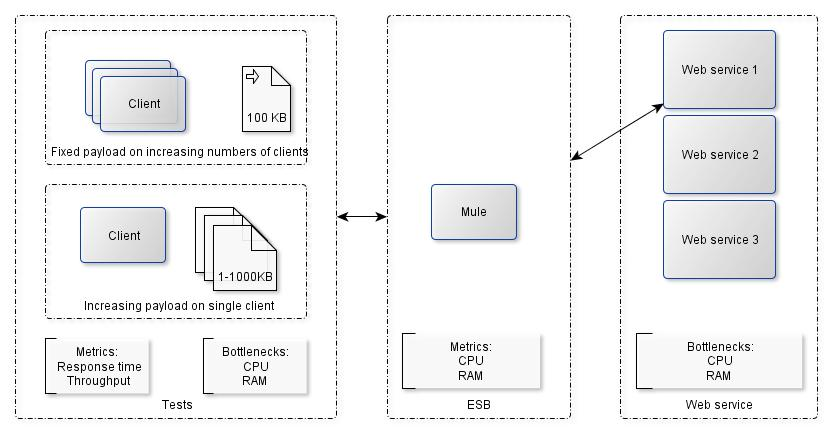
\includegraphics[scale=0.43]{img/direct_proxy}}

\subsection{Routing}
In this test the ESB will, depending on the context of an incoming request from the Client, send the request to an appropriate web service which will append some data and return the request to the ESB which will send the response to the Client.
This represents the ability to have several systems behind an ESB all showing the same front to the outside.
This test is deemed basic because it is what an should do, separate the systems integration with each other, stepping in as a ``middle-man'' directing requests on behalf of the systems being integrated making the need for changing the systems minimal and just focus on the ESB. 
A test like this could simulate a load balancer where the ESB is a front for two or more systems each running an instance of the same service. Another thing this could simulate is different systems handling different (but similar) data, for example one system behind the ESB is handling user registrations and another one is handling user logins. The ESB can then look at the request payload and decide what user interaction is happening and thus mediate the request to the appropriate system.

\centerline{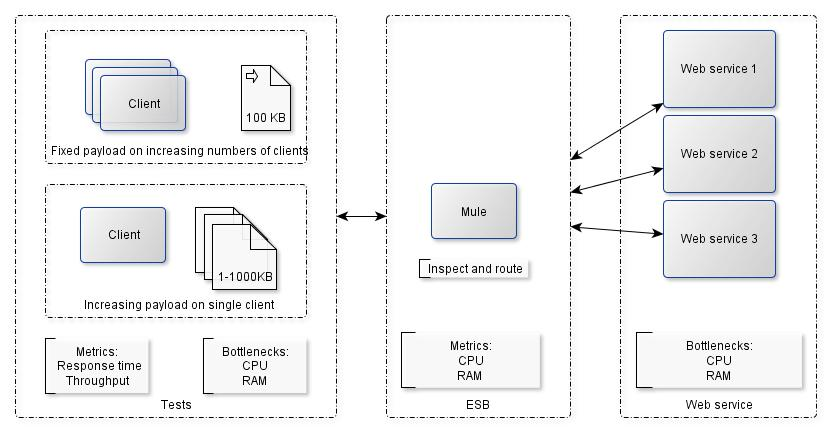
\includegraphics[scale=0.43]{img/Routing}}
\subsection{Message transformation}
The ESB will convert an incoming request to a different format and send it to a web service which will append some data and return the request to the ESB which will transform it back into the format the Client originally sent it.
Transformation is a huge deal for any ESB since two systems to be integrated probably will not speak the same language (XML, json etc) and even if they do they may not have the same format. Of course the systems need to be able to communicate with each others, without an ESB this could become cumbersome since all involved systems would have to be changed in order to understand what the others where saying, just imagine an old system written in COBOL or Assembler and making it communicate with a new system like a web service using REST \cite{whatisrest}. Integration like this cost both money and time and probably won't be future friendly with regards to maintenance.
This could make an ESB invaluable since the ESB would take care of receiving the incoming request in one format, decide where the request is to be sent, transform it to a format which the receiving system can understand, get a response back and transforming it to a format the original system which sent the request will understand.

\centerline{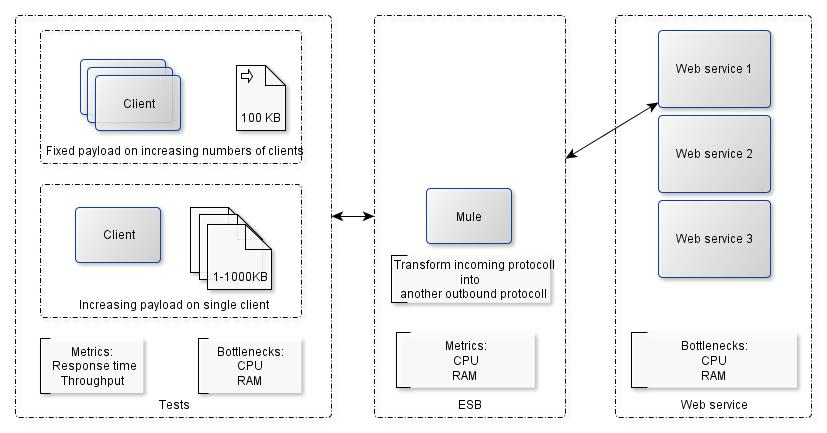
\includegraphics[scale=0.43]{img/transformation}}
\subsection{Artifacts and tools}
\begin{itemize}
	\item Client: Grinder \cite{whatisgrinder, kod}
	\item ESB: Mule \cite{whatismule, kod}
	\item Web service: Jax-WS \cite{whatisjaxws, kod}
	\item OS: Windows 7, 6.1.7600 build 7600
\end{itemize}

\subsection{Hardware setup}
In order to minimize the amount of factors that interfere in the tests we consider having at least three similar state of the art computers, connected to a high-speed network, essential.
It might not be of the greatest importance that the computers are state of the art but in order to not reach a hardware ceiling while testing, such machines are recommended. 
What's most important is that one computer is designated to run ESBs, one is designated to generate traffic(called Client) while the others are simple servers responding to the traffic generated (called Web service). 

% TODO: fixa en lista över hårdvaran (CPU,RAM,HDD osv osv)

This separating and designating of roles to machines minimizes different hardware affecting test results as the same machines perform the same roles in all tests and the only thing changed is the ESB. 

It also means that if other machines are used in other tests the data produced can be compared to ours and as such validate the data or identify faults in the tests. 
This validation can be done in two ways. 
First is to run the same software versions and compare the results. 
They should be similar deviating only in magnitude. The second is if using a newer or old software version the values when put in a graph will either have the same shape or show areas in which performance has changed, 
if it is the same shape but the magnitude is higher then that is most likely caused by faster machines being used and vice versa if its the same magnitude except in certain areas then that shows an improvement in the software.

\subsection{Variables and variable control}
No limitiations has been forseen except for hardware and notwork.
Hardware and network loads should be monitored so they are not close too 100\% as that would mean there is a major bottleneck present. 
All involved computers a run with the same operating system.
\subsection{Experiment schedule and execution sequence}
The three tests have two different focuses. First is to test scalability with an increasing amount of simulated clients (1, 20, 40, 80, 160) sending concurrent requests. 
The other is to test load-handling where a single client will send varying sizes of payload, 1KB, 50KB, 100KB, 500KB and 1MB.
\subsection{Validity threats}
This section discusses different validity threats.
\subsubsection{Different operating systems}
%Different operating system will effect test results 
%TODO säkerställ att unix inte påverkar resultaten nämnvärt
kan påvera men vi kommer att köra testerna på lite olika system så vi har ett hum om vilka förändringar det innebär i datan.
\subsubsection{Different hardware}
%TODO kör testerna en gång på /// så vi inte påverkas för mycket av hårdvara
see "different operating systems"
\subsubsection{Inefficient code}
We are not expert in the various programming languages and systems used to perform these tests and as such our code might be inefficient and even wrong. Inefficient code is not a problem as long as the same code is used in all tests. Erroneous code however is unmaintainable code and as such will require too be changed in the future and that will most likely affect the test results and test history. 
The possibilities of erroneous code has been limited by focusing the tests on very simple and basic functionality that doesn't require expert knowledge of the ESB in order to get results.
By actually providing the source code we have opened up the possibility for improvements and additions of more advanced tests which we feel is extremely important for a consistent testing framework used in academia and industry.
\section{Conclusion}

%1: answer RQs
The current body of knowledge is severely lacking in both academia and industry. We found only two papers \cite{Sanjay2011,Garcia2010} doing performance tests in academia and a larger number of outdated and biased industrial papers \cite{Perera07,Perera07R2,Perera07R3,mulesoft08}.
There is enough papers for us to at least get a foundation of testing to build upon which is what we do in our test framework. The framework consists of a series of scenarios aimed at testing the core functionality of any ESB and we have used Mule ESB as verification that the framework works as expected. 

%2:	our contribution
The largest conclusion done in this thesis is that the current body of knowledge seems to be severly lacking in both industry and academia. 
Most importantly the paper we have found \cite{Sanjay2011} lack a reproducibility which is, possibly, even more important than an unbiased test. 
We have also started a humble attempt at creating a testing framework that could serve as a foundation for future tests. 
Below is an analysis of some of the other tests performed byt others and how they compare to our results.


\newpage

\begin{figure}[H]
	\caption{Image taken from WSO2s test \cite{Perera07R3} showing their content based routing measurements.}
	\centerline{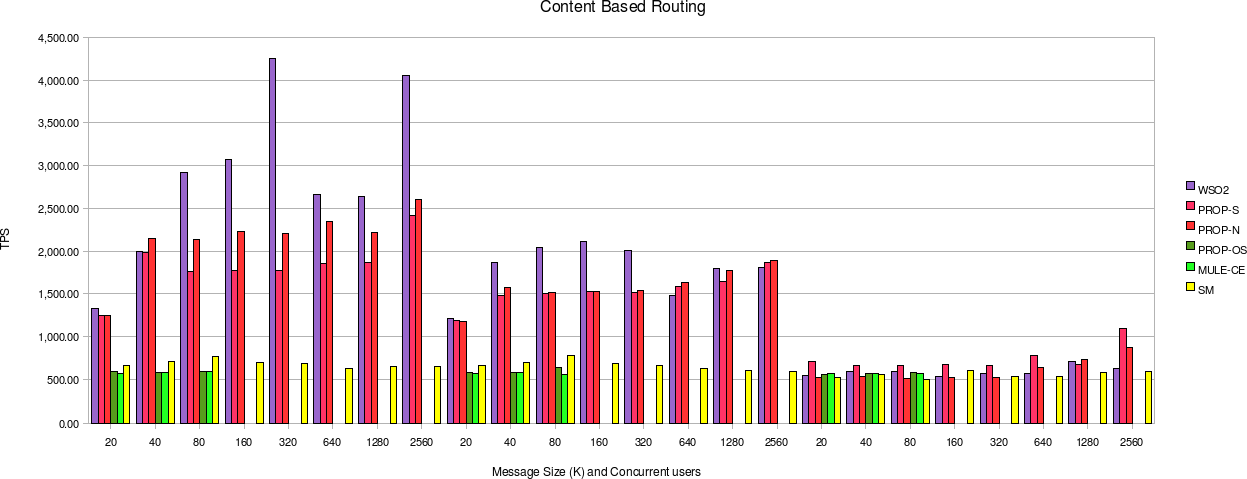
\includegraphics[scale=0.43]{img/WSO2_cbr_chart}}
	\label{fig:wso2_cbr}
	Payload is increasing (0.5KB, 1KB and 5KB) and the X-axis is numbers of clients sending data. 
	All values seem to be above 500TPS with some tests not being able to complete on all ESB solutions.

	\caption{Image taken from Mules test \cite{mulesoft08} showing their content based routing measurements.}
	\centerline{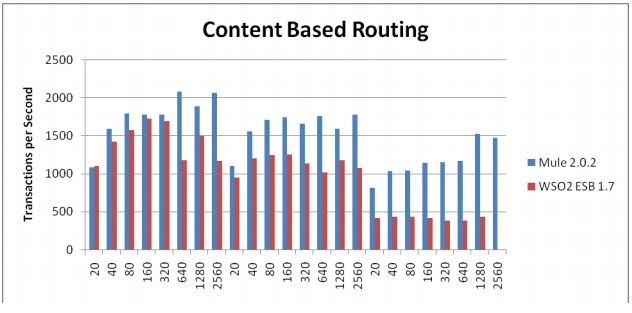
\includegraphics[scale=1]{img/MULE_cbr_chart}}
	\label{fig:mule_cbr}
	Payload is increasing (0.5KB, 1KB and 5KB) and the X-axis is numbers of clients sending data. 
\end{figure}
While looking at figure \ref{fig:wso2_cbr} we can clearly see that Mule has failed the majority of tests performed by WSO2 \cite{Perera07R3}. 
It is therefore not suprising that in the following figure from Mules test \cite{mulesoft08} shows WSO2 failing tests and performing far below Mule.
This blame-game is why it's so important to have a unified performance testing framework that everyone can use as a performance index that can be trusted for its accuracy and unbiased measuring.

What is most suprising to us is that in these tests the TPS is above 500TPS and often above 1000TPS overall. 
If we look at the second "20" mark on the x-axis which is 1KB sent by 20 concurrent users both WSO2 and Mules tests show values between 500TPS and 1000TPS while in our own tests with an ESB didn't even break 10TPS.
Even without an ESB we could not achieve such high numbers which could mean that the configuration of grinder or the webservice needs to be finetuned.

\newpage

\begin{figure}[H]
	\caption{Image taken from Sanjay \cite{Sanjay2011} showing their fixed payload content based routing measurements.}
	\centerline{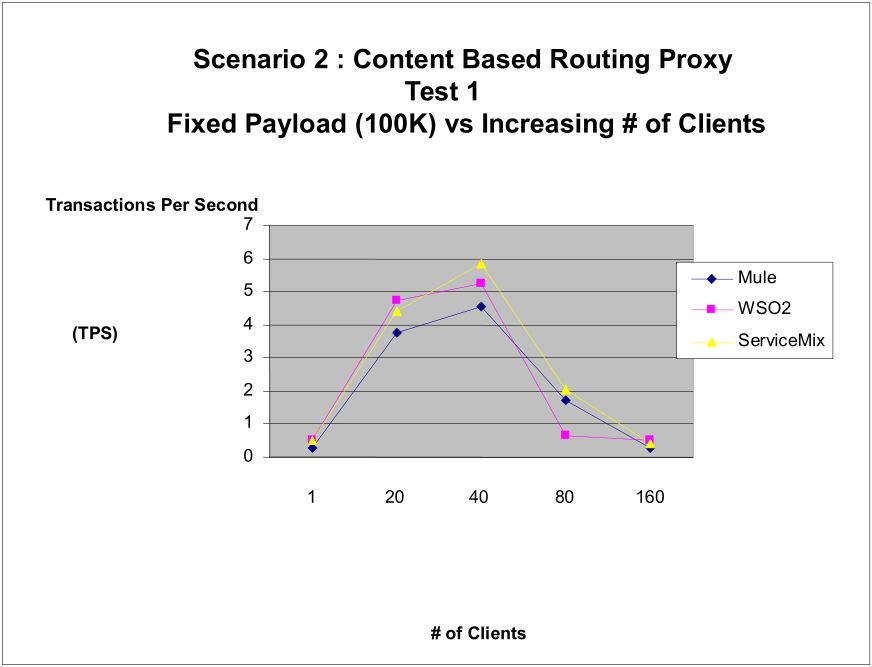
\includegraphics[scale=0.43]{img/Sanjay_cbr_fixed_payload}}
	\label{fig:sanjay_cbr_fixed_payload}
	Using a fixed payload of 100KB and an increasing number of clients the throughput was peaking at 4.5-6 TPS at 40 concurrent clients.

	\caption{Image taken from Sanjay \cite{Sanjay2011} showing their increasing clients content based routing measurements.}
	\centerline{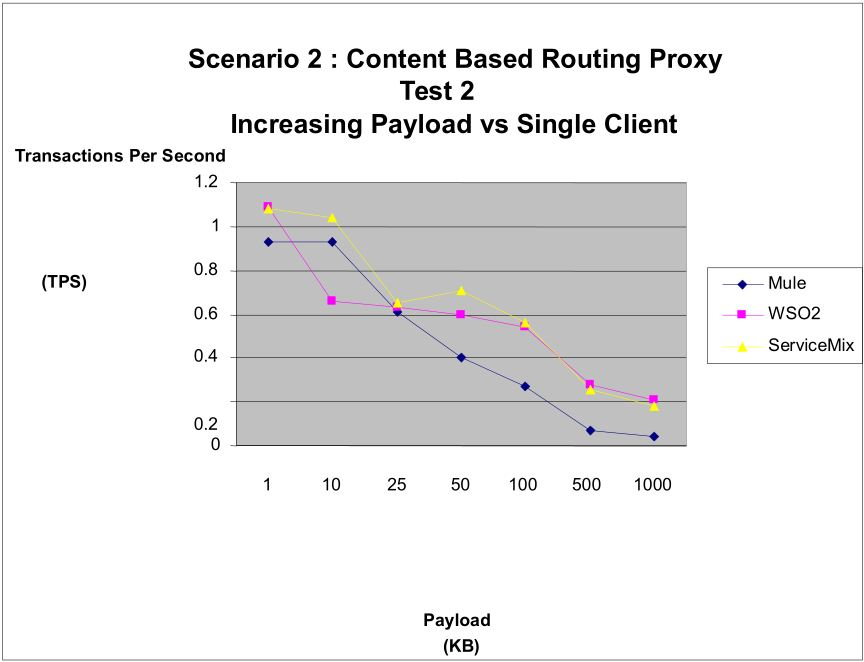
\includegraphics[scale=0.43]{img/Sanjay_cbr_increasing_payload}}
	\label{fig:sanjay_cbr_increasing_payload}
	Single client sending an increasingly larger payload with a TPS between 1.1 and 0.2 which are simply appallingly low numbers.
\end{figure}

When looking at the results from Sanjay \cite{Sanjay2011} in figure \ref{fig:sanjay_cbr_fixed_payload}, \ref{fig:sanjay_cbr_increasing_payload} and the results from WSO2 and Mule \cite{Perera07R3,mulesoft08} in figure \ref{fig:wso2_cbr} and \ref{fig:mule_cbr} one can't help but wonder how Sanjay performed their tests.
Even without the knowledge of the previous tests by WSO2 and Mule their numbers are so low that it seems impossible to consider them as correct yet there is no discussion regarding the validity of the data or their testing procedure. 
It doesn't help that they have not published their hardware setup nor their configuration and ESB source code which means that we cant even begin to hypothezise regarding their data. 


Our results as seen in chapter \ref{test:results} indicate to us that the framework needs more finetuning but that it is a good start for future work. 
The largest contribution done in this thesis is that this could be a starting point for making a testing framework that gives reproducable results and a unified way of testing ESB performance.


%3: future work
One of the more interesting suggestions we would like to make is to include the ESB manufacturers themselves and have them produce the ESB code that is then tested using the framework. 
This would allow a larger number of ESBs to be tested and the code would contain less faults due to the testers inexperience of a particular ESB. 
It would require some secrecy as otherwise the ESB manufacturers could optimize the code in an unnatural manner and that would skew the results.

Recieving optimized code from the manufacturers would also create a baseline that could be used inorder for the tests to be made more advanced and complex.
Increased complexity of the tests could result in more accurate performance tests as the hardware is pushed closer to being maxed out.
Some finetuning of the tools used such as grinder could also be required before the framework should be used on a larger scale.

The configuration files and all source code used in the framework can be found on github at https://github.com/Datanizze/korsdrag-thesis-files


\bibliographystyle{ieeetr}
\bibliography{refs}


%\newpage
\section*{Appendices}
\appendix

\section{Grinder configuration}
\label{app:grinder}

\subsection{grinder.properties}
\lstinputlisting{includes/grinder/grinder.properties}

\subsection{grinder\_soap.py}
\lstinputlisting{includes/grinder/grinder_soap.py}

\subsection{grinder\_json.py}
\lstinputlisting{includes/grinder/grinder_json.py}
\newpage
\section{Mule configuration}
\label{app:mule}

\subsection{Initial instructions}
The mule project was created using MuleStudio, a standard empty project where the contents of the flow1.mflow was replaced with the code below.

\subsection{flow1.mflow}
TODO: plocka muleprojektet från filestorage1.bth.se
%\lstinputlisting{includes/mule/flow1.mflow}
\newpage
\section{Web service configuration}
\label{app:webservice}

\subsection{Initial instructions}
Create a regular java project using eclipse and add the following files to the project.

\subsection{WSPublisher.java} 

\lstinputlisting{includes/webservice/WSPublisher.java}

\subsection{EchoService.java} 

\lstinputlisting{includes/webservice/EchoService.java}

\subsection{EchoServiceImpl.java} 

\lstinputlisting{includes/webservice/EchoServiceImpl.java}
\end{document}

